\section{Multiple Integrals}

%%%%%%%%%%%%%%%%%%%%%%
%  Double Integrals  %
%%%%%%%%%%%%%%%%%%%%%%

\subsection{Double Integrals}

If $f(x,y)$ is a function of two variables and $R = [a,b] \times [c,d]$ (that means the ranges for $x$ and $y$ are $a \leq x \leq b$ and $c \leq y \leq d$) is the projection of the region in the $xy$-plane, then we can approximate the volume under the surface $S=f(x,y)$ over the region $R$ as: \[ 
    V \approx \sum_{i=1}^{n} \sum_{j=1}^{m} f(x_i^*,y_j^*) \Delta A_{ij}
\]
where $(x_i^*, y_j^*)$ is a point on the Region $R$ and $\Delta A_{ij}$ is the area of the rectangle in the $xy$-plane with vertices $(x_i,y_j)$, $(x_i,y_{j+1})$, $(x_{i+1},y_j)$, and $(x_{i+1},y_{j+1})$.
We can then take the limit as $n \to \infty$ and $m \to \infty$ to get the volume as \[ 
    V = \lim_{n,m \to \infty} \sum_{i=1}^{n} \sum_{j=1}^{m} f(x_i^*,y_j^*) \Delta A_{ij}
\]

\begin{figure}[htpb]
    \centering
    \begin{subfigure}[t]{0.4\textwidth}
        \centering
        
\includegraphics[width=0.8\textwidth]{4.1.1.png}
        \caption{}
    \end{subfigure}
    \begin{subfigure}[t]{0.4\textwidth}
        \centering
        
\includegraphics[width=0.8\textwidth]{4.1.2.png}
        \caption{}
    \end{subfigure}
    \caption{}
\end{figure}

\Note[Double Integral]{
    \[ \text{Volume} = \iint\limits_R f(x,y) \dd{A} \]
    We can use this double sum in the definition to estimate the value of the double indegral. We can do so by choosing $(x_i^*,y_j^*)$ to be the midpoint of the rectangle $(\bar{x_i},\bar{y_j})$. This leads us to the \textbf{Midpoint Rule} for double integrals:
    \[ 
        \iint\limits_R f(x,y) \dd{A} \approx \sum_{i=1}^{n} \sum_{j=1}^{m} f(\bar{x_i},\bar{y_j}) \Delta A_{ij}
    \]
}

%%%%%%%%%%%%%%%%%%%%%%%%
%  Iterated Integrals  %
%%%%%%%%%%%%%%%%%%%%%%%%

\subsection{Iterated Integrals}

\Theorem{Fubini's Theorem}{
    If $f(x,y)$ is continuous on the rectangle $R = [a,b] \times [c,d]$, then
    \[
        \iint\limits_R f(x,y) \dd{A} = \int_c^d \int_a^b f(x,y) \dd{x} \dd{y} = \int_a^b \int_c^d f(x,y) \dd{y} \dd{x}
    \]
    These integrals are called \textbf{iterated integrals}.
}

\Note{
    If $f(x,y) = g(x)h(y)$ and we're integrating over the rectangle $R = [a,b]\times[c,d]$, then \[ 
        \iint \limits_R f(x,y) \dd{A} = \iint \limits_R g(x)h(y) \dd{A} = \int_a^b g(x) \dd{x} \int_c^d h(y) \dd{y}
    \]
}

\Example{Evaluate $\displaystyle \iint \limits_{R} x \cos^2(y) \dd{A}, R = [-2,3] \times [0, \frac{\pi}{2}]$}{
    Since the integrand is a function of $x$ times a function of $y$, we can use the fact.
    \begin{align*}
        \iint \limits_{R} x \cos^2(y) \dd{x} &= \left( \int_{-2}^{3} x \dd{x} \right) \left( \int_{0}^{\pi/2} \cos^2(y) \dd{y} \right) \\
        &= \left( \frac{1}{2}x^2 \right) \Biggr|_{-2}^{3} \left( \frac{1}{2} \int_{0}^{\pi/2} (1 + \cos(2y)) \dd{y} \right) \\
        &= \frac{5}{4} \left( y + \frac{1}{2} \sin(2y) \right) \Biggr|_{0}^{\pi/2} \\
        &= \frac{5\pi}{8}
    \end{align*}
}

\Example{Determine the volume that lies under $f(x,y) = 9x^2 + 4xy + 4$ and above the rectangle given by $[-1,1] \times [0,2]$ in the $xy$-plane}{
    \begin{align*}
        V &= \iint \limits_{R} (9x^2 + 4xy + 4) \dd{A} \\
          &= \int_{0}^{2} \int_{-1}^{1} (9x^2 + 4xy + 4) \dd{x} \dd{y} \\
          &= \int_{0}^{2} \left( 3x^3 + 2x^2 y + 4x \right) \Bigr|_{-1}^{1} \dd{y} \\
          &= \int_{0}^{2} \left( (3 + 2y + 4) - (-3 + 2y - 4) \right) \dd{y} \\
          &= \int_{0}^{2} (6 + 8) \dd{y} = 14y \Bigr|_{0}^{2} = 28
    \end{align*}
}

%%%%%%%%%%%%%%%%%%%%%%%%%%%%%%%%%%%%%%%%%%%%%%%%%%%%%%%%%%%%%
%  Single Indefinite Integrals of a Multivariable Function  %
%%%%%%%%%%%%%%%%%%%%%%%%%%%%%%%%%%%%%%%%%%%%%%%%%%%%%%%%%%%%%

\subsection{Single Indefinite Integrals of a Multivariable Function}

\Note[Single Indefinite Integral of a Multivariable Function]{
    Let $f(x,y)$ be a function of two variables. Then the \textbf{single indefinite integral} of $f$ with respect to $x$ is given by \[ 
        \int f(x,y) \dd{x} = F(x,y) + C(y)
    \]
    where $F(x,y)$ is any function such that $\pdv{F}{x} = f(x,y)$ and $C(y)$ is any function of $y$. \\
    Similarly, the single indefinite integral of $f$ with respect to $y$ is given by \[ 
        \int f(x,y) \dd{y} = G(x,y) + D(x)
    \]
    where $G(x,y)$ is any function such that $\pdv{G}{y} = f(x,y)$ and $D(x)$ is any function of $x$.
}

\Example{Evaluate $\displaystyle \int (x^2 y + 3xy^2) \dd{x}$ and $\displaystyle \int (x^2 y + 3xy^2) \dd{y}$}{
    \begin{align*}
        \int (x^2 y + 3xy^2) \dd{x} &= \int x^2 y \dd{x} + \int 3xy^2 \dd{x} \\
                                    &= y \int x^2 \dd{x} + 3y^2 \int x \dd{x} \\
                                    &= y \left( \frac{1}{3} x^3 \right) + 3y^2 \left( \frac{1}{2} x^2 \right) + C(y) \\
                                    &= \frac{1}{3} x^3 y + \frac{3}{2} x^2 y^2 + C(y)
    \end{align*}
    \begin{align*}
        \int (x^2 y + 3xy^2) \dd{y} &= \int x^2 y \dd{y} + \int 3xy^2 \dd{y} \\
                                    &= x^2 \int y \dd{y} + 3x \int y^2 \dd{y} \\
                                    &= x^2 \left( \frac{1}{2} y^2 \right) + 3x \left( \frac{1}{3} y^3 \right) + D(x) \\
                                    &= \frac{1}{2} x^2 y^2 + x y^3 + D(x)
    \end{align*}
}

%%%%%%%%%%%%%%%%%%%%%%%%%%%%%%%%%%%%%%%%%%%
%  Double Integrals Over General Regions  %
%%%%%%%%%%%%%%%%%%%%%%%%%%%%%%%%%%%%%%%%%%%

\subsection{Double Integrals Over General Regions}

In previous section, double integrals over rectangular regions were discussed. But most regions are not rectangular, so we need to look at the following double integral now:
\[ 
    \iint \limits_{D} f(x,y) \dd{A}
\]

There are two types of regions that we need to look at. Here are diagrams for both cases:

We can use set builder method to describe these regions as follows:
\begin{itemize}
    \item Case 1: $D = \{ (x,y) | a \leq x \leq b, g_1(x) \leq y \leq g_2(x) \}$
    \item Case 2: $D = \{ (x,y) | c \leq y \leq d, h_1(y) \leq x \leq h_2(y) \}$
\end{itemize}

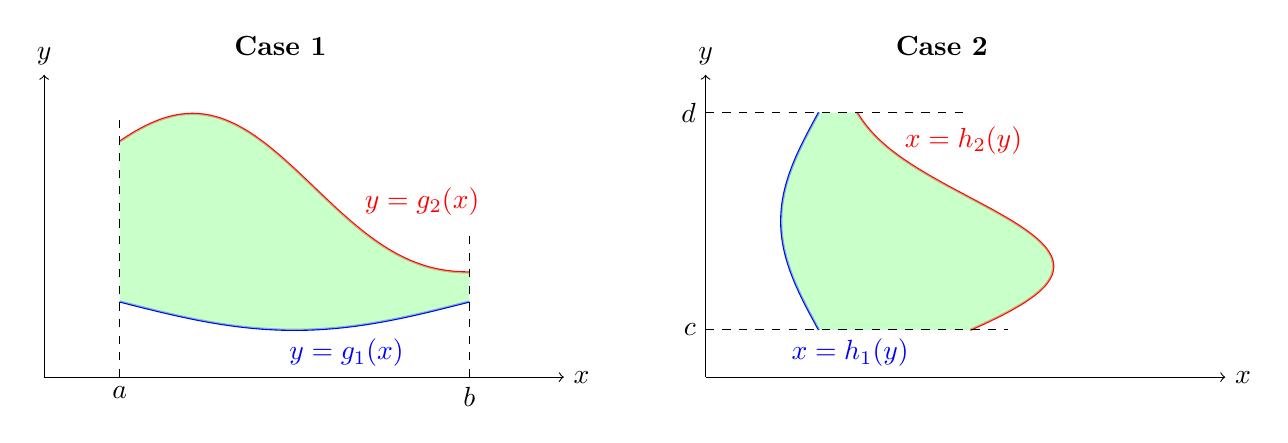
\begin{tikzpicture}[scale=1.2]
    % Case 1
    \begin{scope}[shift={(0,0)}]
        % Title
        \node at (2.5, 3.5) {\textbf{Case 1}};
        % Axes
        \draw[->] (0,0) -- (5.5,0) node[right] {$x$};
        \draw[->] (0,0) -- (0,3.2) node[above] {$y$};
        % Define the curves using smooth plots
        \draw[blue, thick] plot[smooth, domain=0.8:4.5] 
            (\x, {0.8 - 0.3*sin((\x-0.8)*180/3.7)}) node[above] at (3.2,0) {$y=g_1(x)$};
        \draw[red, thick] plot[smooth, domain=0.8:4.5] 
            (\x, {1.8 + 0.8*sin((\x-0.8)*180/3.7 + 60) + 0.2*sin((\x-0.8)*360/3.7)}) 
            node[above] at (4,1.6) {$y=g_2(x)$};
        % Fill the region
        \fill[green!30, opacity=0.7] plot[smooth, domain=0.8:4.5] 
            (\x, {0.8 - 0.3*sin((\x-0.8)*180/3.7)}) 
            -- plot[smooth, domain=4.5:0.8] 
            (\x, {1.8 + 0.8*sin((\x-0.8)*180/3.7 + 60) + 0.2*sin((\x-0.8)*360/3.7)}) 
            -- cycle;
        % Vertical dashed lines
        \draw[dashed] (0.8,0) -- (0.8, 2.8);
        \draw[dashed] (4.5,0) -- (4.5, 1.5);
        % Labels for a and b
        \node[below] at (0.8,0) {$a$};
        \node[below] at (4.5,0) {$b$};
    \end{scope}
    % Case 2
    \begin{scope}[shift={(7,0)}]
        % Title
        \node at (2.5, 3.5) {\textbf{Case 2}};
        % Axes
        \draw[->] (0,0) -- (5.5,0) node[right] {$x$};
        \draw[->] (0,0) -- (0,3.2) node[above] {$y$};
        % Define the curves - now as functions of y
        % Left curve (blue)
        \draw[blue, thick] plot[smooth, domain=0.5:2.8] 
            ({1.2 - 0.4*sin((\x-0.5)*180/2.3)}, \x) node[above right] at (0.8,0) {$x=h_1(y)$};
        % Right curve (red)  
        \draw[red, thick] plot[smooth, domain=0.5:2.8] 
            ({2.2 + 1.2*sin((\x-0.5)*180/2.3 + 30) + 0.3*sin((\x-0.5)*360/2.3)}, \x) 
            node[right] at (2,2.5) {$x=h_2(y)$};
        % Fill the region
        \fill[green!30, opacity=0.7] plot[smooth, domain=0.5:2.8] 
            ({1.2 - 0.4*sin((\x-0.5)*180/2.3)}, \x)
            -- plot[smooth, domain=2.8:0.5] 
            ({2.2 + 1.2*sin((\x-0.5)*180/2.3 + 30) + 0.3*sin((\x-0.5)*360/2.3)}, \x)
            -- cycle;
        % Horizontal dashed lines
        \draw[dashed] (0,0.5) -- (3.2, 0.5);
        \draw[dashed] (0,2.8) -- (2.8, 2.8);
        % Labels for c and d
        \node[left] at (0,0.5) {$c$};
        \node[left] at (0,2.8) {$d$};
    \end{scope}
\end{tikzpicture}

\Note{
    The double integral for both of these cases are defined in terms of iterated integrals as follows:
    \begin{itemize}
        \item Case 1: $D = \{ (x,y) | a \leq x \leq b, g_1(x) \leq y \leq g_2(x) \}$
            \[ 
                \iint \limits_{D} f(x,y) \dd{A} = \int_{a}^{b} \int_{g_1(x)}^{g_2(x)} f(x,y) \dd{y} \dd{x}
            \]
        \item Case 2: $D = \{ (x,y) | c \leq y \leq d, h_1(y) \leq x \leq h_2(y) \}$
            \[ 
                \iint \limits_{D} f(x,y) \dd{A} = \int_{c}^{d} \int_{h_1(y)}^{h_2(y)} f(x,y) \dd{x} \dd{y}
            \]
    \end{itemize}
}

\Note[Properties]{
    \begin{enumerate}
        \item $\displaystyle \iint \limits_{D} \left( f(x,y) + g(x,y) \right) \dd{A} = \iint \limits_{D} f(x,y) \dd{A} + \iint \limits_{D} g(x,y) \dd{A}$
        \item $\displaystyle \iint \limits_{D} k f(x,y) \dd{A} = k \iint \limits_{D} f(x,y) \dd{A}$
        \item If the region $D$ can be split into two separate regions $D_1$ and $D_2$ then the integral can be written as \[ 
            \iint \limits_{D} f(x,y) \dd{A} = \iint \limits_{D_1} f(x,y) \dd{A} + \iint \limits_{D_2} f(x,y) \dd{A}
        \]
    \end{enumerate}
}

\Example{Evaluate the integral $\displaystyle \iint \limits_{D} (6x^2 - 40y) \dd{A}$, where $D$ is the triangle with vertices $(0,3)$, $(1,1)$, and $(5,3)$}{
    We can break the region into two parts and evaluate the integral as follows: \\
    \begin{minipage}{0.6\textwidth}
        \begin{align*}
            D_1 &= \{ (x,y) | 0 \leq x \leq 1, -2x + 3 \leq y \leq 3 \} \\
            D_2 &= \{ (x,y) | 1 \leq x \leq 5, \frac{1}{2}x + \frac{1}{2} \leq y \leq 3 \}
        \end{align*}
    \end{minipage}\hfill
    \begin{minipage}{0.4\textwidth}
        \centering
        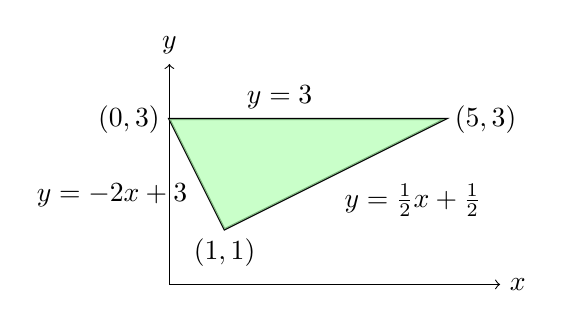
\begin{tikzpicture}[scale=0.7]
        % Axes
            \draw[->] (0,0) -- (6,0) node[right] {$x$};
            \draw[->] (0,0) -- (0,4) node[above] {$y$};
        % Triangle
            \draw[thick] (0,3) -- (1,1) -- (5,3) -- cycle;
        % Labels for vertices
            \node[left] at (0,3) {$(0,3)$};
            \node[below] at (1,1) {$(1,1)$};
            \node[right] at (5,3) {$(5,3)$};
        % Shaded region
            \fill[green!30, opacity=0.7] (0,3) -- (1,1) -- (5,3) -- cycle;
        % Equation of lines
            \node[above] at (2,3) {$y=3$};
            \node[below left] at (0.5,2) {$y=-2x+3$};
            \node[below right] at (3,2) {$y=\frac{1}{2}x+\frac{1}{2}$};
        \end{tikzpicture}
    \end{minipage}

    \textbf{Solution 1:}
    \begin{align*}
        \iint \limits_{D} (6x^2 - 40y) \dd{A} &= \iint \limits_{D_1} (6x^2-40y) \dd{A} + \iint \limits_{D_2} (6x^2-40y) \dd{A} \\
                                              &= \int_{0}^{1} \int_{-2x+3}^{3} (6x^2-40y) \dd{y} \dd{x} + \int_{1}^{5} \int_{\frac{1}{2}x+\frac{1}{2}}^{3} (6x^2-40y) \dd{y} \dd{x} \\
                                              &= \int_{0}^{1} (6x^2y-20y^2)\Bigr|_{-2x+3}^{3} \dd{x} + \int_{1}^{5} (6x^2y-20y^2)\Bigr|_{\frac{1}{2}x+\frac{1}{2}}^{3} \dd{x} \\
                                              &= \int_{0}^{1} (12x^3 - 180 + 20(3-2x)^2) \dd{x} \\
                                              &\quad+ \int_{1}^{5} \left( -3x^3 + 25x^2 - 180 + 20 \left( \frac{1}{2}x + \frac{1}{2} \right)^2 \right) \dd{x} \\
                                              &= \left( 3x^4 - 180x - \frac{10}{3} (3-2x)^3 \right)\Biggr|_{0}^{1} \\
                                              &\quad+ \left( \frac{-3}{4}x^4 + 5x^3 - 180x + \frac{40}{3} \left( \frac{1}{2}x + \frac{1}{2} \right)^3 \right)\Biggr|_{1}^{5} \\
                                              &= -\frac{935}{3}
    \end{align*}
    However, we can also evaluate the integral using a different approach. \\
    \textbf{Solution 2:}
    \begin{align*}
        \iint \limits_{D} (6x^2-40y) \dd{A} &= \int_{1}^{3} \int_{-\frac{1}{2}y+\frac{3}{2}}^{2y-1} (6x^2-40y) \dd{x} \dd{y} \\
                                            &= \int_{1}^{3} (2x^3 - 40xy) \Bigr|_{-\frac{1}{2}y+\frac{3}{2}}^{2y-1} \dd{y} \\
                                            &= \int_{1}^{3} \left[ 100y - 100y^2 + 2(2y-1)^3 - 2 \left( - \frac{1}{2}y + \frac{3}{2} \right)^3 \right] \dd{y} \\
                                            &= \left[ 50y^2 - \frac{100}{3}y^3 + \frac{1}{4}(2y-1)^4 + \left( - \frac{1}{2}y + \frac{3}{2} \right)^4 \right]\Biggr|_{1}^{3} \\
                                            &= -\frac{935}{3}
    \end{align*}
}

\Example{Find the volume of the solid that lies below the surface given by $z=16xy+200$ and lies above the region in the $xy$-plane bounded by $y=x^2$ and $y=8-x^2$.}{
    \vspace{-0.5cm}
    \begin{center}
        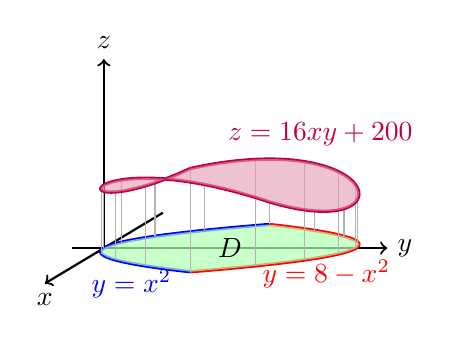
\begin{tikzpicture}[scale=0.5,
            x={(-0.5cm,-0.3cm)}, y={(0.8cm,0cm)}, z={(0cm,0.8cm)}]
            % Axes
            \draw[->, thick] (-3,0,0) -- (3,0,0) node[below] {$x$};
            \draw[->, thick] (0,-1,0) -- (0,9,0) node[right] {$y$};
            \draw[->, thick] (0,0,0) -- (0,0,6) node[above] {$z$};
            % Draw the region D boundary in xy-plane
            \draw[blue, very thick] plot[smooth, domain=-2:2, samples=40] (\x, {\x*\x}, 0);
            \draw[red, very thick] plot[smooth, domain=-2:2, samples=40] (\x, {8-\x*\x}, 0);
            % Close the region at x=-2 and x=2
            \draw[blue, very thick] (-2, 4, 0) -- (-2, 4, 0);
            \draw[blue, very thick] (2, 4, 0) -- (2, 4, 0);
            % Fill the region D in xy-plane
            \fill[green!30, opacity=0.7] plot[smooth, domain=-2:2, samples=40] (\x, {\x*\x}, 0)
                -- plot[smooth, domain=2:-2, samples=40] (\x, {8-\x*\x}, 0) -- cycle;
            % Sample vertical lines showing the solid
            \foreach \xval in {-2,-1.5,-1,-0.5,0,0.5,1,1.5,2} {
                \pgfmathsetmacro{\ybot}{\xval*\xval}
                \pgfmathsetmacro{\ytop}{8-\xval*\xval}
                \pgfmathsetmacro{\zbot}{0.01*(16*\xval*\ybot+200)}
                \pgfmathsetmacro{\ztop}{0.01*(16*\xval*\ytop+200)}
                \draw[gray!60, thin] (\xval, \ybot, 0) -- (\xval, \ybot, \zbot);
                \draw[gray!60, thin] (\xval, \ytop, 0) -- (\xval, \ytop, \ztop);
            }
            % Draw the surface z=16xy+200 boundary curves (scaled down by factor of 100)
            \draw[purple, very thick] plot[smooth, domain=-2:2, samples=40] 
                (\x, {\x*\x}, {0.01*(16*\x*\x*\x+200)});
            \draw[purple, very thick] plot[smooth, domain=-2:2, samples=40] 
                (\x, {8-\x*\x}, {0.01*(16*\x*(8-\x*\x)+200)});
            % Fill the top surface
            \fill[purple!40, opacity=0.6] plot[smooth, domain=-2:2, samples=40] 
                (\x, {\x*\x}, {0.01*(16*\x*\x*\x+200)})
                -- plot[smooth, domain=2:-2, samples=40] 
                (\x, {8-\x*\x}, {0.01*(16*\x*(8-\x*\x)+200)}) -- cycle;
            % Labels for curves in xy-plane
            \node[blue, below] at (1.0, 1.5, 0) {$y=x^2$};
            \node[red, above] at (1.5, 8, -1) {$y=8-x^2$};
            \node at (0, 4, 0) {$D$};
            \node[purple] at (-3, 5, 2.5) {$z=16xy+200$};
        \end{tikzpicture}
    \end{center}
    The volume is given by
    \begin{align*}
        V &= \iint \limits_{D} (16xy+200) \dd{A} \\
          &= \int_{-2}^{2} \int_{x^2}^{8-x^2} (16xy+200) \dd{y} \dd{x} \\
          &= \int_{-2}^{2} (8xy^2+200y)\Bigr|_{x^2}^{8-x^2} \dd{x} \\
          &= \int_{-2}^{2} ( -128x^3 - 400x^2 + 512x + 1600 ) \dd{x} \\
          &= \left( -32x^4 - \frac{400}{3}x^3 + 256x^2 + 1600x \right)\Biggr|_{-2}^{2} \\
          &= \frac{12800}{3}
    \end{align*}
}

\Note{
    In general, \[ 
       V = \iint \limits_{D} f(x,y) \dd{A}
    \]
    gives the net volume between the graph of $z=f(x,y)$ and the region $D$ in the $xy$-plane. Regions that are below the $xy$-plane, have a negative volume, and the regions that are above the $xy$-plane, have a positive volume.
}

\Note{
    \[ 
       \text{Area of region } D = \iint \limits_{D} \dd{A}
    \]
}

%%%%%%%%%%%%%%%%%%%%%%%%%%%%%%%%%%%%%%%%%%%
%  Double Integrals in Polar Coordinates  %
%%%%%%%%%%%%%%%%%%%%%%%%%%%%%%%%%%%%%%%%%%%

\subsection{Double Integrals in Polar Coordinates}

Some regions are much easier to describe in terms of polar coordinates rather than Cartesian coordinates. For instance, we might have a region that is a disk, ring, or a portion of a disk or ring.

\begin{figure}[h]
    \centering
    \begin{subfigure}{0.35\textwidth}
        
\includegraphics[width=\textwidth]{4.5.1.png}
    \end{subfigure}
    \begin{subfigure}{0.60\textwidth}
        
\includegraphics[width=\textwidth]{4.5.2.png}
    \end{subfigure}
    \caption{A region in polar coordinates and its mesh approximation}
    \label{fig:polar_mesh}
\end{figure}

In Figure~\ref{fig:polar_mesh}, the region is broke up into a mesh of radial lines and arcs. The area of each piece is $\Delta A$. Two sides of the piece both have length $\Delta r = r_o - r_i$. And the other two sides are arcs $r_o \Delta\theta$ and $r_i \Delta\theta$. We can assume that the mesh is so small that $r_i \approx r_o \approx r$. Hence, the area of each piece is approximately \[ 
    \Delta A \approx r \Delta r \Delta \theta \implies \dd{A} = r \dd{r} \dd{\theta}
\]
\Note{\vspace{-0.2cm}
    \[ \dd{A} = r \dd{r} \dd{\theta} \]
}
\Note[Polar Rectangle and Area Element]{
    A \textbf{polar rectangle} $R$ is a region in the plane defined by \[
        R = \{ (r, \theta) \mid a \leq r \leq b, \alpha \leq \theta \leq \beta \}
    \]
    where $0 \leq \beta - \alpha \leq 2\pi$. \\
}

\Note[Double Integral for General Polar Regions]{
    For general regions in polar coordinates, if $D = \{ (r, \theta) \mid \alpha \leq \theta \leq \beta, h_1(\theta) \leq r \leq h_2(\theta) \}$, then
    \[
        \iint\limits_D f(x,y) \dd{A} = \int_{\alpha}^{\beta} \int_{h_1(\theta)}^{h_2(\theta)} f(r\cos\theta, r\sin\theta) \, r \dd{r} \dd{\theta}
    \]
}

\Example{Evaluate $\displaystyle \iint\limits_R (3x + 4y^2) \dd{A}$, where $R$ is the region in the upper half-plane bounded by the circles $x^2 + y^2 = 1$ and $x^2 + y^2 = 4$.}{
    The region $R$ can be described in polar coordinates as
    \[
        R = \left\{ (r, \theta) \mid 1 \leq r \leq 2, 0 \leq \theta \leq \pi \right\}
    \]
    Converting to polar coordinates: $x = r\cos\theta$ and $y = r\sin\theta$, and $\dd{A} = r \dd{r} \dd{\theta}$.
    \begin{align*}
        \iint\limits_R (3x + 4y^2) \dd{A} &= \int_{0}^{\pi} \int_{1}^{2} (3r\cos\theta + 4r^2\sin^2\theta) r \dd{r} \dd{\theta} \\
        &= \int_{0}^{\pi} \int_{1}^{2} (3r^2\cos\theta + 4r^3\sin^2\theta) \dd{r} \dd{\theta} \\
        &= \int_{0}^{\pi} \left( r^3\cos\theta + r^4\sin^2\theta \right)\Bigr|_{1}^{2} \dd{\theta} \\
        &= \int_{0}^{\pi} \left( (8\cos\theta + 16\sin^2\theta) - (\cos\theta + \sin^2\theta) \right) \dd{\theta} \\
        &= \int_{0}^{\pi} (7\cos\theta + 15\sin^2\theta) \dd{\theta} \\
        &= \int_{0}^{\pi} \left( 7\cos\theta + 15 \cdot \frac{1 - \cos(2\theta)}{2} \right) \dd{\theta} \\
        &= \left( 7\sin\theta + \frac{15}{2}\theta - \frac{15}{4}\sin(2\theta) \right)\Biggr|_{0}^{\pi} \\
        &= \left( 0 + \frac{15\pi}{2} - 0 \right) - (0 + 0 - 0) = \frac{15\pi}{2}
    \end{align*}
}

\Example{Find the volume of the solid that lies under the paraboloid $z = x^2 + y^2$ and above the disk $x^2 + y^2 \leq 9$.}{
    In polar coordinates, the disk is $D = \{ (r, \theta) \mid 0 \leq r \leq 3, 0 \leq \theta \leq 2\pi \}$ and $z = x^2 + y^2 = r^2$.
    \begin{align*}
        V &= \iint\limits_D (x^2 + y^2) \dd{A} = \int_{0}^{2\pi} \int_{0}^{3} r^2 \cdot r \dd{r} \dd{\theta} \\
        &= \int_{0}^{2\pi} \int_{0}^{3} r^3 \dd{r} \dd{\theta} = \int_{0}^{2\pi} \left( \frac{r^4}{4} \right)\Biggr|_{0}^{3} \dd{\theta} \\
        &= \int_{0}^{2\pi} \frac{81}{4} \dd{\theta} = \frac{81}{4} \cdot 2\pi = \frac{81\pi}{2}
    \end{align*}
}

\Example{Evaluate $\displaystyle \iint\limits_D e^{x^2+y^2} \dd{A}$, where $D$ is the region bounded by the semicircle $x = \sqrt{4-y^2}$ and the $y$-axis in the first quadrant.}{
    The region $D$ is a quarter circle of radius 2 in the first quadrant. In polar coordinates:
    \[
        D = \left\{ (r, \theta) \mid 0 \leq r \leq 2, 0 \leq \theta \leq \frac{\pi}{2} \right\}
    \]
    Since $x^2 + y^2 = r^2$, we have $e^{x^2+y^2} = e^{r^2}$.
    \begin{align*}
        \iint\limits_D e^{x^2+y^2} \dd{A} &= \int_{0}^{\pi/2} \int_{0}^{2} e^{r^2} \cdot r \dd{r} \dd{\theta}
    \end{align*}
    Using the substitution $u = r^2$, so $\dd{u} = 2r \dd{r}$:
    \begin{align*}
        &= \int_{0}^{\pi/2} \left( \frac{1}{2} \int_{0}^{4} e^{u} \dd{u} \right) \dd{\theta} \\
        &= \int_{0}^{\pi/2} \frac{1}{2} \left( e^{u} \right)\Bigr|_{0}^{4} \dd{\theta} \\
        &= \int_{0}^{\pi/2} \frac{1}{2}(e^4 - 1) \dd{\theta} \\
        &= \frac{e^4 - 1}{2} \cdot \frac{\pi}{2} = \frac{\pi(e^4-1)}{4}
    \end{align*}
}

\Note[When to Use Polar Coordinates]{
    Polar coordinates are particularly useful when:
    \begin{enumerate}
        \item The region $D$ is a circle, disk, annulus, or sector of a circle
        \item The function $f(x,y)$ can be simplified using $x^2 + y^2 = r^2$ (e.g., $f(x,y) = \sqrt{x^2+y^2}$ becomes $f(r,\theta) = r$)
        \item The integrand contains expressions like $x^2 + y^2$, $\sqrt{x^2+y^2}$, or $\arctan(y/x)$
    \end{enumerate}
}

%%%%%%%%%%%%%%%%%%%%%%
%  Triple Integrals  %
%%%%%%%%%%%%%%%%%%%%%%

\subsection{Triple Integrals}

Triple integrals extend the concept of double integrals to three dimensions. Just as double integrals compute volumes under surfaces in 2D regions, triple integrals can compute various quantities over three-dimensional regions, including volumes and masses.

\Note[Triple Integral]{
    For a function $f(x,y,z)$ defined over a three-dimensional region $E$, the triple integral is denoted:
    \[
        \iiint \limits_{E} f(x,y,z) \dd{V}
    \]
    where $\dd{V} = \dd{x}\dd{y}\dd{z}$ represents the differential volume element.
}

\Note[Volume of 3D Region]{
    The volume of a three-dimensional region $E$ is given by the triple integral
    \[
        V = \iiint \limits_{E} \dd{V}
    \]
}

\Note[Triple Integrals over Boxes]{
    For a rectangular box $B = [a,b] \times [c,d] \times [r,s]$, the triple integral can be evaluated as an iterated integral
    \[
        \iiint \limits_{B} f(x,y,z) \dd{V} = \int_{r}^{s} \int_{c}^{d} \int_{a}^{b} f(x,y,z) \dd{x}\dd{y}\dd{z} \\
    \]
}

\Example{Evaluate $\displaystyle \iiint \limits_{B} 8xyz^2 \dd{V}$ where $B = [1,2] \times [0,1] \times [-1,1]$.}{
    We can use any order of integration. Let's use $\dd{x}\dd{y}\dd{z}$:
    \begin{align*}
        \iiint \limits_{B} 8xyz^2 \dd{V} &= \int_{-1}^{1} \int_{0}^{1} \int_{1}^{2} 8xyz^2 \dd{x}\dd{y}\dd{z} \\
        &= \int_{-1}^{1} \int_{0}^{1} 4x^2yz^2\Bigr|_{x=1}^{x=2} \dd{y}\dd{z} \\
        &= \int_{-1}^{1} \int_{0}^{1} (16yz^2 - 4yz^2) \dd{y}\dd{z} \\
        &= \int_{-1}^{1} \int_{0}^{1} 12yz^2 \dd{y}\dd{z} \\
        &= \int_{-1}^{1} 6y^2z^2\Bigr|_{y=0}^{y=1} \dd{z} \\
        &= \int_{-1}^{1} 6z^2 \dd{z} \\
        &=  2z^3\Bigr|_{-1}^{1} \\
        &= 2(1) - 2(-1) = 4
    \end{align*}
}


% Triple Integrals over General Regions %

\subsubsection{Triple Integrals over General Regions}

For more general regions, we define three types of regions that allow us to set up triple integrals with variable limits.

\begin{figure}[h]
    \centering
    \begin{subfigure}{0.3\textwidth}
        
\includegraphics[width=\textwidth]{4.6.1.png}
    \end{subfigure}
    \begin{subfigure}{0.3\textwidth}
        
\includegraphics[width=\textwidth]{4.6.2.png}
    \end{subfigure}
    \begin{subfigure}{0.3\textwidth}
        
\includegraphics[width=\textwidth]{4.6.3.png}
    \end{subfigure}
    \caption{Types I, II, and III regions for triple integrals}
    \label{fig:triple_integral_over_general_region}
\end{figure}

\Note[Type I Region]{
    A solid region $E$ is of \textbf{Type I} if it lies between the graphs of two continuous functions of $x$ and $y$:
    \[
        E = \{(x,y,z) \mid (x,y) \in D, \, u_1(x,y) \leq z \leq u_2(x,y)\}
    \]
    where $D$ is the projection of $E$ onto the $xy$-plane.
    
    For such regions:
    \[
        \iiint \limits_{E} f(x,y,z) \dd{V} = \iint \limits_{D} \left[ \int_{u_1(x,y)}^{u_2(x,y)} f(x,y,z) \dd{z} \right] \dd{A}
    \]
}

\Note[Type II Region]{
    A solid region $E$ is of \textbf{Type II} if it lies between the graphs of two continuous functions of $y$ and $z$:
    \[
        E = \{(x,y,z) \mid (y,z) \in D, \, u_1(y,z) \leq x \leq u_2(y,z)\}
    \]
    where $D$ is the projection of $E$ onto the $yz$-plane.
    
    For such regions:
    \[
        \iiint \limits_{E} f(x,y,z) \dd{V} = \iint \limits_{D} \left[ \int_{u_1(y,z)}^{u_2(y,z)} f(x,y,z) \dd{x} \right] \dd{A}
    \]
}

\Note[Type III Region]{
    A solid region $E$ is of \textbf{Type III} if it lies between the graphs of two continuous functions of $x$ and $z$:
    \[
        E = \{(x,y,z) \mid (x,z) \in D, \, u_1(x,z) \leq y \leq u_2(x,z)\}
    \]
    where $D$ is the projection of $E$ onto the $xz$-plane.
    
    For such regions:
    \[
        \iiint \limits_{E} f(x,y,z) \dd{V} = \iint \limits_{D} \left[ \int_{u_1(x,z)}^{u_2(x,z)} f(x,y,z) \dd{y} \right] \dd{A}
    \]
}

\Example{Find the volume of the tetrahedron bounded by the plane $x + 2y + z = 2$ and the coordinate planes.}{
    This is a Type I region. First, we need to find the projection $D$ onto the $xy$-plane. The plane intersects:
    \begin{itemize}
        \item $x$-axis at $(2,0,0)$ when $y=z=0$
        \item $y$-axis at $(0,1,0)$ when $x=z=0$
        \item $z$-axis at $(0,0,2)$ when $x=y=0$
    \end{itemize}
    The projection $D$ onto the $xy$-plane is the triangle with vertices $(0,0)$, $(2,0)$, and $(0,1)$, bounded by:
    \begin{itemize}
        \item $x = 0$ (the $y$-axis)
        \item $y = 0$ (the $x$-axis)
        \item $x + 2y = 2$ (or $y = \frac{2-x}{2}$)
    \end{itemize}
    For a Type I region, $z$ ranges from the lower surface $z = 0$ to the upper surface $z = 2 - x - 2y$. \\
    The volume is:
    \begin{align*}
        V &= \iiint \limits_{E} \dd{V} = \int_{0}^{2} \int_{0}^{(2-x)/2} \int_{0}^{2-x-2y} \dd{z} \dd{y} \dd{x} \\
        &= \int_{0}^{2} \int_{0}^{(2-x)/2} [z]_{0}^{2-x-2y} \dd{y} \dd{x} \\
        &= \int_{0}^{2} \int_{0}^{(2-x)/2} (2-x-2y) \dd{y} \dd{x} \\
        &= \int_{0}^{2} \left[ (2-x)y - y^2 \right]_{0}^{(2-x)/2} \dd{x} \\
        &= \int_{0}^{2} \left[ (2-x) \cdot \frac{2-x}{2} - \left(\frac{2-x}{2}\right)^2 \right] \dd{x} \\
        &= \int_{0}^{2} \left[ \frac{(2-x)^2}{2} - \frac{(2-x)^2}{4} \right] \dd{x} \\
        &= \int_{0}^{2} \frac{(2-x)^2}{4} \dd{x} \\
        &= \frac{1}{4} \int_{0}^{2} (2-x)^2 \dd{x}
    \end{align*}
    Let $u = 2-x$, so $\dd{u} = -\dd{x}$. When $x=0$, $u=2$; when $x=2$, $u=0$:
    \begin{align*}
        V &= \frac{1}{4} \int_{2}^{0} u^2 (-\dd{u}) = \frac{1}{4} \int_{0}^{2} u^2 \dd{u} \\
        &= \frac{1}{4} \left[ \frac{u^3}{3} \right]_{0}^{2} = \frac{1}{4} \cdot \frac{8}{3} = \frac{2}{3}
    \end{align*}
}

\Example{Evaluate $\displaystyle \iiint \limits_{E} z \dd{V}$ where $E$ is bounded by $y = 0$, $z = 0$, $y = x$, and $x + z = 1$ in the first octant.}{
    This region is bounded by four planes. Let's use a Type II approach where we integrate with respect to $x$ first. \\
    The region can be described as:
    \begin{itemize}
        \item The projection onto the $yz$-plane is bounded by $z = 0$, $y = 0$, $y + z \leq 1$
        \item For each $(y,z)$ in this projection, $x$ ranges from $y$ to $1-z$
    \end{itemize}
    However, we need $y \leq 1-z$ for the region to exist, which gives us $y \leq 1-z$. \\
    Setting up as Type I (integrating $z$ first) is easier:
    \begin{itemize}
        \item Project onto the $xy$-plane: the region is bounded by $y = 0$, $y = x$, and $x \leq 1$
        \item For each $(x,y)$, $z$ ranges from $0$ to $1-x$
    \end{itemize}
    \begin{align*}
        \iiint \limits_{E} z \dd{V} &= \int_{0}^{1} \int_{0}^{x} \int_{0}^{1-x} z \dd{z} \dd{y} \dd{x} \\
        &= \int_{0}^{1} \int_{0}^{x} \left[ \frac{z^2}{2} \right]_{0}^{1-x} \dd{y} \dd{x} \\
        &= \int_{0}^{1} \int_{0}^{x} \frac{(1-x)^2}{2} \dd{y} \dd{x} \\
        &= \int_{0}^{1} \frac{(1-x)^2}{2} [y]_{0}^{x} \dd{x} \\
        &= \int_{0}^{1} \frac{x(1-x)^2}{2} \dd{x} \\
        &= \frac{1}{2} \int_{0}^{1} x(1-2x+x^2) \dd{x} \\
        &= \frac{1}{2} \int_{0}^{1} (x - 2x^2 + x^3) \dd{x} \\
        &= \frac{1}{2} \left[ \frac{x^2}{2} - \frac{2x^3}{3} + \frac{x^4}{4} \right]_{0}^{1} \\
        &= \frac{1}{2} \left( \frac{1}{2} - \frac{2}{3} + \frac{1}{4} \right) \\
        &= \frac{1}{2} \left( \frac{6 - 8 + 3}{12} \right) = \frac{1}{2} \cdot \frac{1}{12} = \frac{1}{24}
    \end{align*}
}

%%%%%%%%%%%%%%%%%%%%%%%%%%%%%%%%%%%%%%%%%%%%%%%%%
%  Triple Integrals in Cylindrical Coordinates  %
%%%%%%%%%%%%%%%%%%%%%%%%%%%%%%%%%%%%%%%%%%%%%%%%%

\subsection{Triple Integrals in Cylindrical Coordinates}

Cylindrical coordinates are an extension of polar coordinates into three dimensions, making them particularly useful for regions with circular symmetry about the $z$-axis.

\Note[Recall: Cylindrical Coordinates]{
    The cylindrical coordinate system is defined by:
    \[
        x = r\cos\theta, \quad y = r\sin\theta, \quad z = z
    \]
    where $r \geq 0$ is the distance from the $z$-axis, $\theta$ is the angle from the positive $x$-axis, and $z$ is the height.
    
    The volume element in cylindrical coordinates is:
    \[
        \dd{V} = r\dd{z}\dd{r}\dd{\theta}
    \]
}

\Note[Triple Integral in Cylindrical Coordinates]{
    For a region $E$ where $(x,y) \in D$ in the $xy$-plane and $u_1(x,y) \leq z \leq u_2(x,y)$, the triple integral becomes:
    \[
        \iiint \limits_{E} f(x,y,z) \dd{V} = \int_{\alpha}^{\beta} \int_{h_1(\theta)}^{h_2(\theta)} \int_{u_1(r\cos\theta,r\sin\theta)}^{u_2(r\cos\theta,r\sin\theta)} f(r\cos\theta, r\sin\theta, z) \cdot r \dd{z}\dd{r}\dd{\theta}
    \]
}

\Example{Evaluate $\displaystyle \iiint \limits_{E} y \dd{V}$ where $E$ is the region below $z = x+2$, above the $xy$-plane, and between the cylinders $x^2+y^2=1$ and $x^2+y^2=4$.}{
    First, convert the bounds to cylindrical coordinates:
    \begin{itemize}
        \item The plane $z = x + 2$ becomes $z = r\cos\theta + 2$
        \item Above the $xy$-plane means $z \geq 0$
        \item Between cylinders: $1 \leq r \leq 2$
        \item Full rotation: $0 \leq \theta \leq 2\pi$
    \end{itemize}
    
    Converting $y = r\sin\theta$:
    \begin{align*}
        \iiint \limits_{E} y \dd{V} &= \int_{0}^{2\pi} \int_{1}^{2} \int_{0}^{r\cos\theta+2} r(r\sin\theta) \dd{z}\dd{r}\dd{\theta} \\
        &= \int_{0}^{2\pi} \int_{1}^{2} r^2\sin\theta (r\cos\theta + 2) \dd{r}\dd{\theta} \\
        &= \int_{0}^{2\pi} \int_{1}^{2} \left( r^3\sin\theta\cos\theta + 2r^2\sin\theta \right) \dd{r}\dd{\theta} \\
        &= \int_{0}^{2\pi} \int_{1}^{2} \left( \frac{1}{2}r^3\sin(2\theta) + 2r^2\sin\theta \right) \dd{r}\dd{\theta} \\
        &= \int_{0}^{2\pi} \left[ \frac{1}{8}r^4\sin(2\theta) + \frac{2}{3}r^3\sin\theta \right]_{1}^{2} \dd{\theta} \\
        &= \int_{0}^{2\pi} \left( \frac{15}{8}\sin(2\theta) + \frac{14}{3}\sin\theta \right) \dd{\theta} \\
        &= \left[ -\frac{15}{16}\cos(2\theta) - \frac{14}{3}\cos\theta \right]_{0}^{2\pi} \\
        &= 0
    \end{align*}
}

%%%%%%%%%%%%%%%%%%%%%%%%%%%%%%%%%%%%%%%%%%%%%%%%%
%  Triple Integrals in Spherical Coordinates    %
%%%%%%%%%%%%%%%%%%%%%%%%%%%%%%%%%%%%%%%%%%%%%%%%%

\subsection{Triple Integrals in Spherical Coordinates}

Spherical coordinates are particularly useful for regions with spherical symmetry, such as spheres, cones, and combinations thereof.

\begin{figure}[h]
    \centering
    
\includegraphics[width=0.3\textwidth]{4.8.1.png}
    \caption{Spherical coordinates representation}
    \label{fig:spherical_coordinates}
\end{figure}

\Note[Recall: Spherical Coordinates]{
    The spherical coordinate system is defined by: \[
        x = \rho\sin\varphi\cos\theta, \quad y = \rho\sin\varphi\sin\theta, \quad z = \rho\cos\varphi
    \] \[
        x^2 + y^2 + z^2 = \rho^2
    \]
    where:
    \begin{itemize}
        \item $\rho \geq 0$ is the distance from the origin
        \item $\theta$ is the angle in the $xy$-plane from the positive $x$-axis ($0 \leq \theta \leq 2\pi$)
        \item $\varphi$ is the angle from the positive $z$-axis ($0 \leq \varphi \leq \pi$)
    \end{itemize}
    The volume element in spherical coordinates is:
    \[
        \dd{V} = \rho^2\sin\varphi \dd{\rho}\dd{\theta}\dd{\varphi}
    \]
}

\Note[Triple Integral in Spherical Coordinates]{
    For a spherical wedge with $a \leq \rho \leq b$, $\alpha \leq \theta \leq \beta$, and $\delta \leq \varphi \leq \gamma$:
    \[
        \iiint \limits_{E} f(x,y,z) \dd{V} = \int_{\delta}^{\gamma} \int_{\alpha}^{\beta} \int_{a}^{b} f(\rho\sin\varphi\cos\theta, \rho\sin\varphi\sin\theta, \rho\cos\varphi) \cdot \rho^2\sin\varphi \dd{\rho}\dd{\theta}\dd{\varphi}
    \]
}

\Example{Evaluate $\displaystyle \iiint \limits_{E} 16z \dd{V}$ where $E$ is the upper half of the sphere $x^2+y^2+z^2=1$.}{
    The upper half of the unit sphere has limits:
    \begin{itemize}
        \item $0 \leq \rho \leq 1$ (radius from 0 to 1)
        \item $0 \leq \theta \leq 2\pi$ (full rotation)
        \item $0 \leq \varphi \leq \frac{\pi}{2}$ (upper half, from $z$-axis to $xy$-plane)
    \end{itemize}
    Converting $z = \rho\cos\varphi$:
    \begin{align*}
        \iiint \limits_{E} 16z \dd{V} &= \int_{0}^{\pi/2} \int_{0}^{2\pi} \int_{0}^{1} \rho^2\sin\varphi (16\rho\cos\varphi) \dd{\rho}\dd{\theta}\dd{\varphi} \\
        &= \int_{0}^{\pi/2} \int_{0}^{2\pi} \int_{0}^{1} 16\rho^3\sin\varphi\cos\varphi \dd{\rho}\dd{\theta}\dd{\varphi} \\
        &= \int_{0}^{\pi/2} \int_{0}^{2\pi} \int_{0}^{1} 8\rho^3\sin(2\varphi) \dd{\rho}\dd{\theta}\dd{\varphi} \\
        &= \int_{0}^{\pi/2} \int_{0}^{2\pi} 2\sin(2\varphi) \dd{\theta}\dd{\varphi} \\
        &= \int_{0}^{\pi/2} 4\pi\sin(2\varphi) \dd{\varphi} \\
        &= \left[ -2\pi\cos(2\varphi) \right]_{0}^{\pi/2} \\
        &= -2\pi(-1) - (-2\pi)(1) = 4\pi
    \end{align*}
}

\Example{Evaluate $\displaystyle \iiint \limits_{E} zx \dd{V}$ where $E$ is inside $x^2+y^2+z^2=4$ and the upward-pointing cone making angle $\frac{\pi}{3}$ with the negative $z$-axis, with $x \leq 0$.}{
    This region is an upside-down ice cream cone, cut in half with $x \leq 0$ remaining. \\
    Setting up the limits:
    \begin{itemize}
        \item $0 \leq \rho \leq 2$ (inside sphere of radius 2)
        \item $\frac{\pi}{2} \leq \theta \leq \frac{3\pi}{2}$ (left half-plane where $x \leq 0$)
        \item The cone makes angle $\frac{\pi}{3}$ with negative $z$-axis, so from positive $z$-axis it's at angle $\pi - \frac{\pi}{3} = \frac{2\pi}{3}$, giving $\frac{2\pi}{3} \leq \varphi \leq \pi$
    \end{itemize}
    \begin{align*}
        \iiint \limits_{E} zx \dd{V} &= \int_{2\pi/3}^{\pi} \int_{\pi/2}^{3\pi/2} \int_{0}^{2} (\rho\cos\varphi)(\rho\sin\varphi\cos\theta) \rho^2\sin\varphi \dd{\rho}\dd{\theta}\dd{\varphi} \\
        &= \int_{2\pi/3}^{\pi} \int_{\pi/2}^{3\pi/2} \int_{0}^{2} \rho^4\cos\varphi\sin^2\varphi\cos\theta \dd{\rho}\dd{\theta}\dd{\varphi} \\
        &= \int_{2\pi/3}^{\pi} \int_{\pi/2}^{3\pi/2} \frac{32}{5}\cos\varphi\sin^2\varphi\cos\theta \dd{\theta}\dd{\varphi} \\
        &= \int_{2\pi/3}^{\pi} \frac{32}{5}\cos\varphi\sin^2\varphi [\sin\theta]_{\pi/2}^{3\pi/2} \dd{\varphi} \\
        &= \int_{2\pi/3}^{\pi} \frac{32}{5}\cos\varphi\sin^2\varphi (-1-1) \dd{\varphi} \\
        &= -\frac{64}{5} \int_{2\pi/3}^{\pi} \cos\varphi\sin^2\varphi \dd{\varphi} \\
        &= -\frac{64}{5} \left[ \frac{\sin^3\varphi}{3} \right]_{2\pi/3}^{\pi} = -\frac{64}{15} \left( 0 - \frac{3\sqrt{3}}{8} \right) = \frac{8\sqrt{3}}{5}
    \end{align*}
}

%%%%%%%%%%%%%%%%%%%%%%%%%%%%%%%%%%%%%%%%%%%%%%%%%
%  Change of Variables                          %
%%%%%%%%%%%%%%%%%%%%%%%%%%%%%%%%%%%%%%%%%%%%%%%%%

\subsection{Change of Variables}

Just as we had substitution in Calculus I to transform integrals into simpler forms, we can perform similar transformations for double and triple integrals.

% Transformations and Regions %

\subsubsection{Transformations and Regions}

When performing a change of variables, we use a \textbf{transformation} to convert from one coordinate system to another. Typically, we start with a region $R$ in $xy$-coordinates and transform it into a region $S$ in $uv$-coordinates.

\Definition{Transformation}{
    A \textbf{transformation} $T: S \to R$ is given by equations: \[
        x = g(u,v), \quad y = h(u,v)
    \]
    that map points $(u,v)$ in region $S$ to points $(x,y)$ in region $R$.
}

\Example{An ellipse $R$ given by $x^2+\frac{y^2}{36}=1$ transforms into a circle under $x = \frac{u}{2}$, $y = 3v$.}{
    Applying the transformation:
    \begin{align*}
        \left(\frac{u}{2}\right)^2 + \frac{(3v)^2}{36} &= 1 \\
        \frac{u^2}{4} + \frac{9v^2}{36} &= 1 \\
        \frac{u^2}{4} + \frac{v^2}{4} &= 1 \\
        u^2 + v^2 &= 4
    \end{align*}
    
    The ellipse in the $xy$-plane transforms into a disk of radius 2 in the $uv$-plane.
}

% The Jacobian %

\subsubsection{The Jacobian}

The key to changing variables in multiple integrals is the \textbf{Jacobian}, which measures how area or volume scales under the transformation.

\Definition{Jacobian for Double Integrals}{
    The \textbf{Jacobian} of the transformation $x = g(u,v)$, $y = h(u,v)$ is:
    \[
        \frac{\partial(x,y)}{\partial(u,v)} = \begin{vmatrix}
            \pdv{x}{u} & \pdv{x}{v} \\[8pt]
            \pdv{y}{u} & \pdv{y}{v}
        \end{vmatrix} = \pdv{x}{u}\pdv{y}{v} - \pdv{x}{v}\pdv{y}{u}
    \]
}

\Theorem{Change of Variables Formula for Double Integrals}{
    If $T: S \to R$ is a transformation given by $x = g(u,v)$ and $y = h(u,v)$, then:
    \[
        \iint \limits_{R} f(x,y) \dd{A} = \iint \limits_{S} f(g(u,v), h(u,v)) \left| \frac{\partial(x,y)}{\partial(u,v)} \right| \dd{\overline{A}}
    \]
    where $\dd{\overline{A}} = \dd{u}\dd{v}$ in the transformed integral.
    
    Equivalently:
    \[
        \dd{A} = \left| \frac{\partial(x,y)}{\partial(u,v)} \right| \dd{\overline{A}}
    \]
}

\Example{Verify $\dd{A} = r\dd{r}\dd{\theta}$ for polar coordinates.}{
    The polar coordinate transformation is: \[
        x = r\cos\theta, \quad y = r\sin\theta
    \]
    Compute the Jacobian:
    \begin{align*}
        \frac{\partial(x,y)}{\partial(r,\theta)} &= \begin{vmatrix}
            \pdv{x}{r} & \pdv{x}{\theta} \\[8pt]
            \pdv{y}{r} & \pdv{y}{\theta}
        \end{vmatrix}
        = \begin{vmatrix}
            \cos\theta & -r\sin\theta \\
            \sin\theta & r\cos\theta
        \end{vmatrix} \\
        &= r\cos^2\theta - (-r\sin^2\theta) \\
        &= r
    \end{align*}
    Therefore: \[
        \dd{A} = \left| \frac{\partial(x,y)}{\partial(r,\theta)} \right| \dd{r}\dd{\theta} = |r| \dd{r}\dd{\theta} = r\dd{r}\dd{\theta}
    \]
    since $r \geq 0$ in polar coordinates.
}

\Example{Evaluate $\displaystyle \iint \limits_{R} (x+y) \dd{A}$ where $R$ is the trapezoidal region with vertices $(0,0)$, $(5,0)$, $\left(\frac{5}{2}, \frac{5}{2}\right)$, $\left(\frac{5}{2}, -\frac{5}{2}\right)$ using transformation $x = 2u + 3v$, $y = 2u - 3v$.}{
    First, find the equations of the sides of $R$:
    \begin{itemize}
        \item From $(0,0)$ to $\left(\frac{5}{2}, \frac{5}{2}\right)$: $y = x$
        \item From $(0,0)$ to $\left(\frac{5}{2}, -\frac{5}{2}\right)$: $y = -x$
        \item From $\left(\frac{5}{2}, \frac{5}{2}\right)$ to $(5,0)$: $y = -x + 5$
        \item From $\left(\frac{5}{2}, -\frac{5}{2}\right)$ to $(5,0)$: $y = x - 5$
    \end{itemize}
    
    Transform each edge:
    \begin{itemize}
        \item $y = x$: $2u - 3v = 2u + 3v \Rightarrow v = 0$
        \item $y = -x$: $2u - 3v = -(2u + 3v) \Rightarrow u = 0$
        \item $y = -x + 5$: $2u - 3v = -(2u + 3v) + 5 \Rightarrow u = \frac{5}{4}$
        \item $y = x - 5$: $2u - 3v = (2u + 3v) - 5 \Rightarrow v = \frac{5}{6}$
    \end{itemize}
    
    The region $S$ is the rectangle: $0 \leq u \leq \frac{5}{4}$, $0 \leq v \leq \frac{5}{6}$.
    
    Compute the Jacobian:
    \[
        \frac{\partial(x,y)}{\partial(u,v)} = \begin{vmatrix} 2 & 3 \\ 2 & -3 \end{vmatrix} = -6 - 6 = -12
    \]
    
    Evaluate the integral:
    \begin{align*}
        \iint \limits_{R} (x+y) \dd{A} &= \int_{0}^{5/6} \int_{0}^{5/4} [(2u+3v) + (2u-3v)] |-12| \dd{u}\dd{v} \\
        &= \int_{0}^{5/6} \int_{0}^{5/4} 48u \dd{u}\dd{v} \\
        &= \int_{0}^{5/6} \left[ 24u^2 \right]_{0}^{5/4} \dd{v} \\
        &= \int_{0}^{5/6} \frac{75}{2} \dd{v} \\
        &= \frac{75}{2} \cdot \frac{5}{6} = \frac{125}{4}
    \end{align*}
}

% Jacobian for Triple Integrals %

\subsubsection{Jacobian for Triple Integrals}

For triple integrals with transformation $x = g(u,v,w)$, $y = h(u,v,w)$, $z = k(u,v,w)$:

\Definition{Jacobian for Triple Integrals}{
    The \textbf{Jacobian} for a transformation from $(u,v,w)$ to $(x,y,z)$ is:
    \[
        \frac{\partial(x,y,z)}{\partial(u,v,w)} = \begin{vmatrix}
            \pdv{x}{u} & \pdv{x}{v} & \pdv{x}{w} \\[8pt]
            \pdv{y}{u} & \pdv{y}{v} & \pdv{y}{w} \\[8pt]
            \pdv{z}{u} & \pdv{z}{v} & \pdv{z}{w}
        \end{vmatrix}
    \]
}

\Theorem{Change of Variables Formula for Triple Integrals}{
    If $T: S \to R$ transforms region $S$ to region $R$, then:
    \[
        \iiint \limits_{R} f(x,y,z) \dd{V} = \iiint \limits_{S} f(g(u,v,w), h(u,v,w), k(u,v,w)) \left| \frac{\partial(x,y,z)}{\partial(u,v,w)} \right| \dd{\overline{V}}
    \]
    where $\dd{\overline{V}} = \dd{u}\dd{v}\dd{w}$ in the transformed integral. \\
    Equivalently: \[ 
        \dd{V} = \left| \frac{\partial(x,y,z)}{\partial(u,v,w)} \right| \dd{\overline{V}}
    \]
}

\Example{Verify $\dd{V} = \rho^2\sin\varphi \dd{\rho}\dd{\theta}\dd{\varphi}$ for spherical coordinates.}{
    The spherical coordinate transformation is:
    \[
        x = \rho\sin\varphi\cos\theta, \quad y = \rho\sin\varphi\sin\theta, \quad z = \rho\cos\varphi
    \]
    
    Compute the Jacobian:
    \begin{align*}
        \frac{\partial(x,y,z)}{\partial(\rho,\theta,\varphi)} &= \begin{vmatrix}
            \sin\varphi\cos\theta & -\rho\sin\varphi\sin\theta & \rho\cos\varphi\cos\theta \\
            \sin\varphi\sin\theta & \rho\sin\varphi\cos\theta & \rho\cos\varphi\sin\theta \\
            \cos\varphi & 0 & -\rho\sin\varphi
        \end{vmatrix}
    \end{align*}
    
    Expanding along the third row:
    \begin{align*}
        &= \cos\varphi \begin{vmatrix}
            -\rho\sin\varphi\sin\theta & \rho\cos\varphi\cos\theta \\
            \rho\sin\varphi\cos\theta & \rho\cos\varphi\sin\theta
        \end{vmatrix} \\
        &\quad - 0 + (-\rho\sin\varphi) \begin{vmatrix}
            \sin\varphi\cos\theta & -\rho\sin\varphi\sin\theta \\
            \sin\varphi\sin\theta & \rho\sin\varphi\cos\theta
        \end{vmatrix} \\
        &= \cos\varphi(-\rho^2\sin\varphi\cos\varphi\sin^2\theta - \rho^2\sin\varphi\cos\varphi\cos^2\theta) \\
        &\quad + (-\rho\sin\varphi)(\rho\sin^2\varphi\cos^2\theta + \rho\sin^2\varphi\sin^2\theta) \\
        &= -\rho^2\sin\varphi\cos^2\varphi - \rho^2\sin^3\varphi \\
        &= -\rho^2\sin\varphi(\cos^2\varphi + \sin^2\varphi) \\
        &= -\rho^2\sin\varphi
    \end{align*}
    
    Therefore:
    \[
        \dd{V} = \left| -\rho^2\sin\varphi \right| \dd{\rho}\dd{\theta}\dd{\varphi} = \rho^2\sin\varphi \dd{\rho}\dd{\theta}\dd{\varphi}
    \]
    since $\sin\varphi \geq 0$ for $0 \leq \varphi \leq \pi$.
}

% Surface Area %

\subsubsection{Surface Area}

\Note[Surface Area]{
    The surface area $S$ of a surface $z = f(x,y)$ over a region $R$ in the $xy$-plane is given by: \[
        S = \iint \limits_{R} \sqrt{1 + \left( \pdv{f}{x} \right)^2 + \left( \pdv{f}{y} \right)^2} \dd{A}
    \]
}

\Example{Determine the surface area of the part of $z=xy$ that lies in the cylinder given by $x^2+y^2=1$.}{
    First, compute the partial derivatives: \[
        \pdv{f}{x} = y, \quad \pdv{f}{y} = x
    \]
    Given that $D$ is a disk of radius 1, we do this integral in polar coordinates.
    \begin{align*}
        S &= \iint \limits_{D} \sqrt{x^2 + y^2 + 1} \dd{A} \\
          &= \int_{0}^{2\pi} \int_{0}^{1} \sqrt{r^2 + 1} \cdot r \dd{r}\dd{\theta} \\
            &= \int_{0}^{2\pi} \left[ \frac{1}{3}(r^2 + 1)^{3/2} \right]_{0}^{1} \dd{\theta} \\
            &= \int_{0}^{2\pi} \frac{1}{3}(2^{3/2} - 1) \dd{\theta} \\
            &= \frac{2\pi}{3}(2^{3/2} - 1)
    \end{align*}
}
